\documentclass[12pt]{article}
\usepackage[english]{babel}
\usepackage[utf8x]{inputenc}
\usepackage{amsmath}
\usepackage{graphicx}
\usepackage[colorinlistoftodos]{todonotes}
\usepackage{hyperref}

\begin{document}
	
	\begin{titlepage}
		
		\newcommand{\HRule}{\rule{\linewidth}{0.5mm}} % Defines a new command for the horizontal lines, change thickness here
		
		\center % Center everything on the page
		
		%----------------------------------------------------------------------------------------
		%	HEADING SECTIONS
		%----------------------------------------------------------------------------------------
		
		\textsc{\LARGE Ahmedabad University}\\[1.5cm] % Name of your university/college
		\textsc{\Large School of Engineering and Applied Science}\\[0.5cm] % Major heading such as course name
		
		
		%----------------------------------------------------------------------------------------
		%	TITLE SECTION
		%----------------------------------------------------------------------------------------
		
		\HRule \\[0.4cm]
		{ \huge \bfseries Page Replacement Algorithm}\\[0.4cm] % Title of your document
		\HRule \\[1.5cm]
		
		%----------------------------------------------------------------------------------------
		%	AUTHOR SECTION
		%----------------------------------------------------------------------------------------
		
		\begin{minipage}{0.4\textwidth}
			\begin{flushleft} \large
				\emph{Project By:}\\
				Anuj \textsc{Shah} % Your name
				\\Charvik \textsc{Patel}% Your name
				\\Himanshu \textsc{Budhia}% Your name
				\\Maharsh \textsc{Patel}% Your name
			\end{flushleft}
		\end{minipage}
		~
		\begin{minipage}{0.4\textwidth}
			\begin{flushright} \large
				\emph{Instructor:} \\
				Dr. Sanjay \textsc{Choudhary} % Supervisor's Name
				\emph{Mentor:} \\
				Purnima \textsc{Shah} % Supervisor's Name
			\end{flushright}
		\end{minipage}\\[2cm]
		
		% If you don't want a supervisor, uncomment the two lines below and remove the section above
		%\Large \emph{Author:}\\
		%John \textsc{Smith}\\[3cm] % Your name
		
		%----------------------------------------------------------------------------------------
		%	DATE SECTION
		%----------------------------------------------------------------------------------------
		
		{\large \today}\\[2cm] % Date, change the \today to a set date if you want to be precise
		
		%----------------------------------------------------------------------------------------
		%	LOGO SECTION
		%----------------------------------------------------------------------------------------
		
		
\includegraphics{AU.png}\\[0.5cm] % Include a department/university logo - this will require the graphicx package
		
		%----------------------------------------------------------------------------------------
		
		\vfill % Fill the rest of the page with whitespace
		
	\end{titlepage}
	
	
	
	\section{Brief Description}
	The basic idea of Page Replacement is; if there is a free page in the memory then use it. If there is no free page available, then we select one victim page which we would swap out of the virtual memory to the disk. Then we read the desired page to the new free frame. The page tables are then updated and the process is restarted.
	The main objective of a good replacement algorithm is to achieve a low page fault rate. For that we need to insure that the heavily used pages stay in the memory, and the replaced page should not be needed for some time.
	Secondly, we need to reduce the latency of a page fault. That can be assured by writing an efficient code, and replace the pages that do not need to be written out.	
	\section{Flow Chart}
	\includegraphics[height=10cm]{FlowChart.png}
	
	%\section{Flow Chart}
		%\includegraphics{FlowChart.png}
		
		
		
	\section{Algorithm Implementation}
	\subsection{FIFO}
	This Page Replacement Algorithm treats the page frames allocated to a process as a circular buffer:
	\begin{enumerate}
		\item when the buffer is full, the oldest page is replaced. Hence First-in First-out
		\item we require only one pointer, that circles through the page frames of the process.
	\end{enumerate}
	The OS keeps the tracks of all the pages in memory in a queue, with most recent arrival at the back, and the oldest arrival in the front.
	When a page needs to be replaced, the page at the front of the queue(oldest) is selected.

		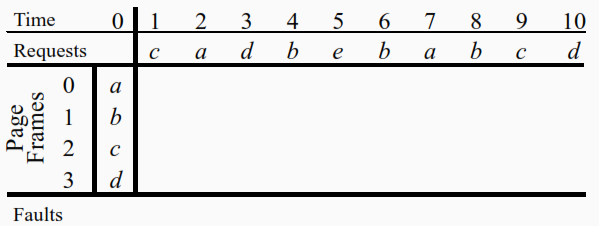
\includegraphics[width=10cm,height=4cm]{FIFO_1}\\
		\centering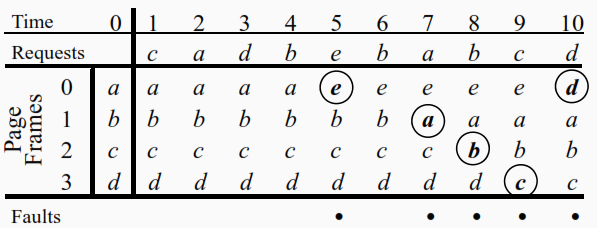
\includegraphics[width=10cm,height=4cm]{FIFO_2}	
		\pagebreak
		\begin{flushleft}
			\subsection{LFU}
		In this Page Replacement Algorithm, we assign a counter to every page. All the counters are initialized by 0. Each time a reference is made to that page, the counter value is incremented by one. When the cache reaches the capacity, and a request for a page that is not present in the memory is made, the system will search for the page with the least number of references (counter value) and replace it from the cache.
		\subsection{LRU Counter}
		\begin{enumerate}
			\item Every page entry has a counter.
			\item Every time a page is referenced, increment a global counter and store it in the page counter.
			\item For replacement, search the page with the lowest counter value and replace it.
		\end{enumerate}
		\subsection{LRU Stack}
		\begin{enumerate}
			\item Maintain a stack of page numbers in a doubly linked list.
			\item When a reference to a page is made, move it to the top of the stack.
			\item For replacement, choose the bottom page.
		\end{enumerate}
		
		\end{flushleft}\pagebreak
		\centering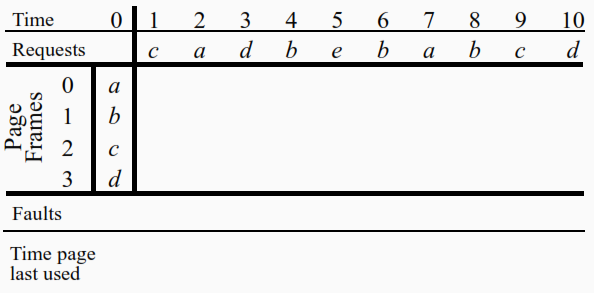
\includegraphics[width=10cm,height=4cm]{LRU_1}\\
		\centering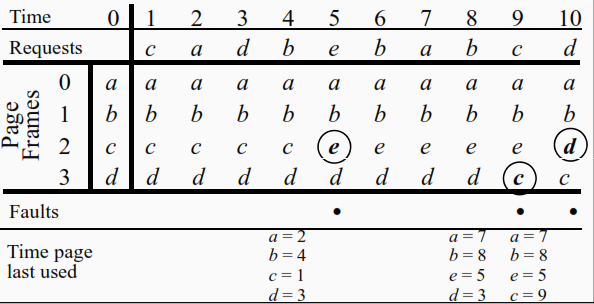
\includegraphics[width=10cm,height=4cm]{LRU_2}\\
		\centering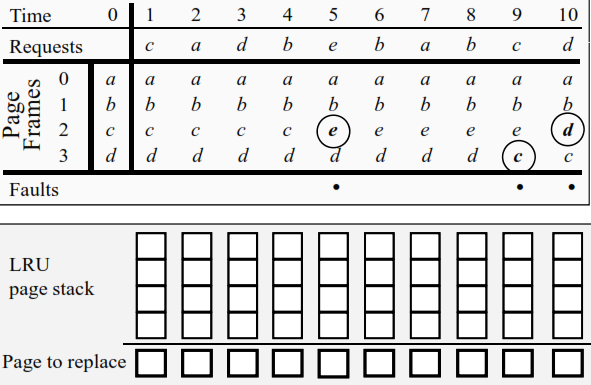
\includegraphics[width=10cm,height=4cm]{LRU_3}\\
		\centering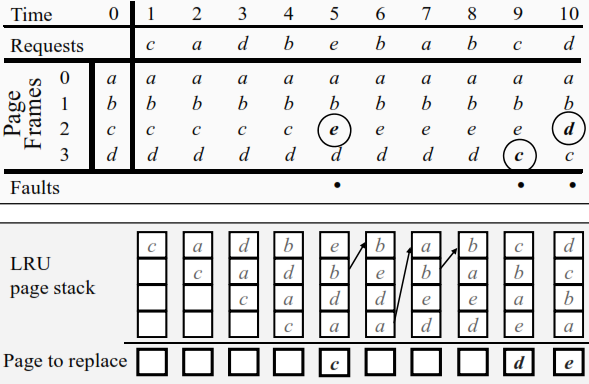
\includegraphics[width=10cm,height=4cm]{LRU_4}\\
		\begin{center}
			Step of LRU
		\end{center}
		\pagebreak
		\begin{flushleft}
			\subsection{MFU}
			In this Page Replacement Algorithm, we assign a counter to every page. All the counters are initialized by 0. Each time a reference is made to that page, the counter value is incremented by one. When the cache reaches the capacity, and a request for a page that is not present in the memory is made, the system will search for the page with the most number of references (counter value) and replace it from the cache.
		\end{flushleft}
			\centering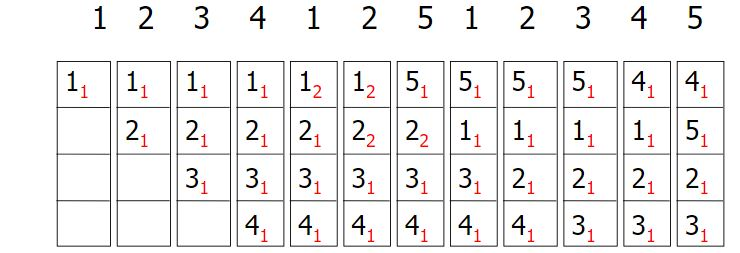
\includegraphics[width=10cm,height=4cm]{MFU_1.JPG}\\
			MFU \\Total Page Fault:10
			\begin{flushleft}
				\subsection{OPT}
				\begin{enumerate}
					\item An optimal page-replacement algorithm has the lowest page-fault rate.
					\item Replace the page that has not been referenced for the longest period of time.
				\end{enumerate}
			\end{flushleft}
			
		
		\centering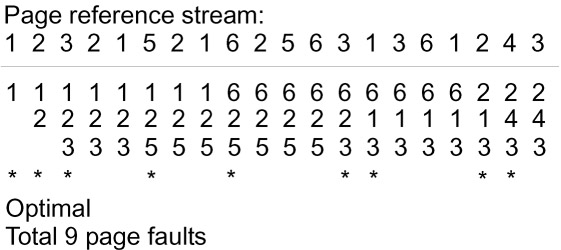
\includegraphics[width=10cm,height=4cm]{OPT_1.png}
		\pagebreak
		\begin{flushleft}
			\subsection{Second Chance}
			\begin{enumerate}
				\item This algorithm is a FIFO replacement algorithm with a small modification that causes it to approximate to LRU.
				\item When a page is selected according to FIFO order, we check its reference bit. If it is set (the page was referenced), we clear it and look for another page.
				
			\end{enumerate}
		\end{flushleft}
		
		
		\centering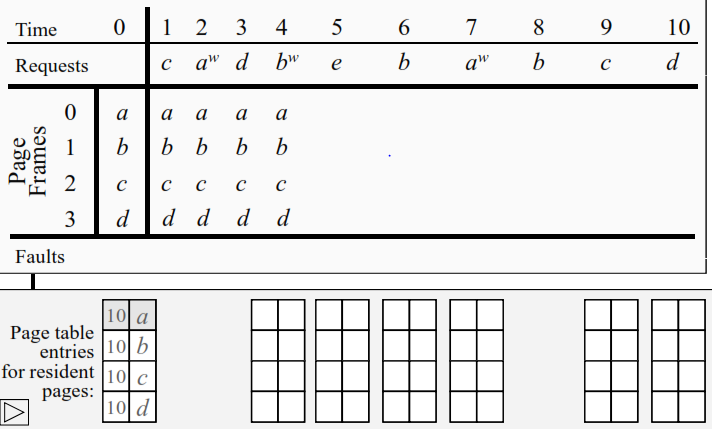
\includegraphics[width=10cm,height=4cm]{SecondChance_1.PNG}
		\centering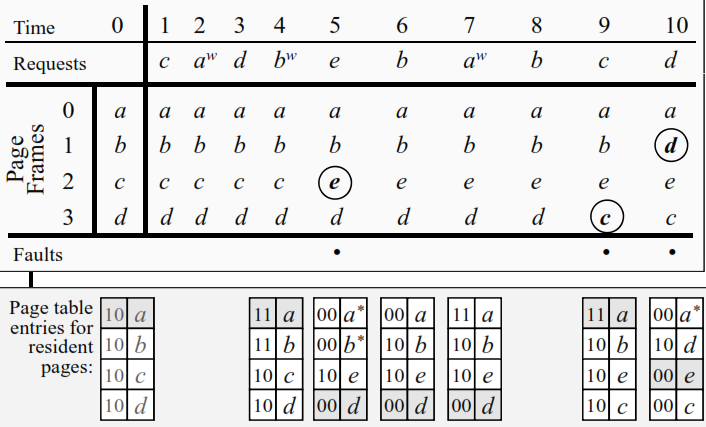
\includegraphics[width=10cm,height=4cm]{SecondChance_2.PNG}
		
		\begin{flushleft}
			\section{Test Result:}
		
		\subsection{FIFO}
		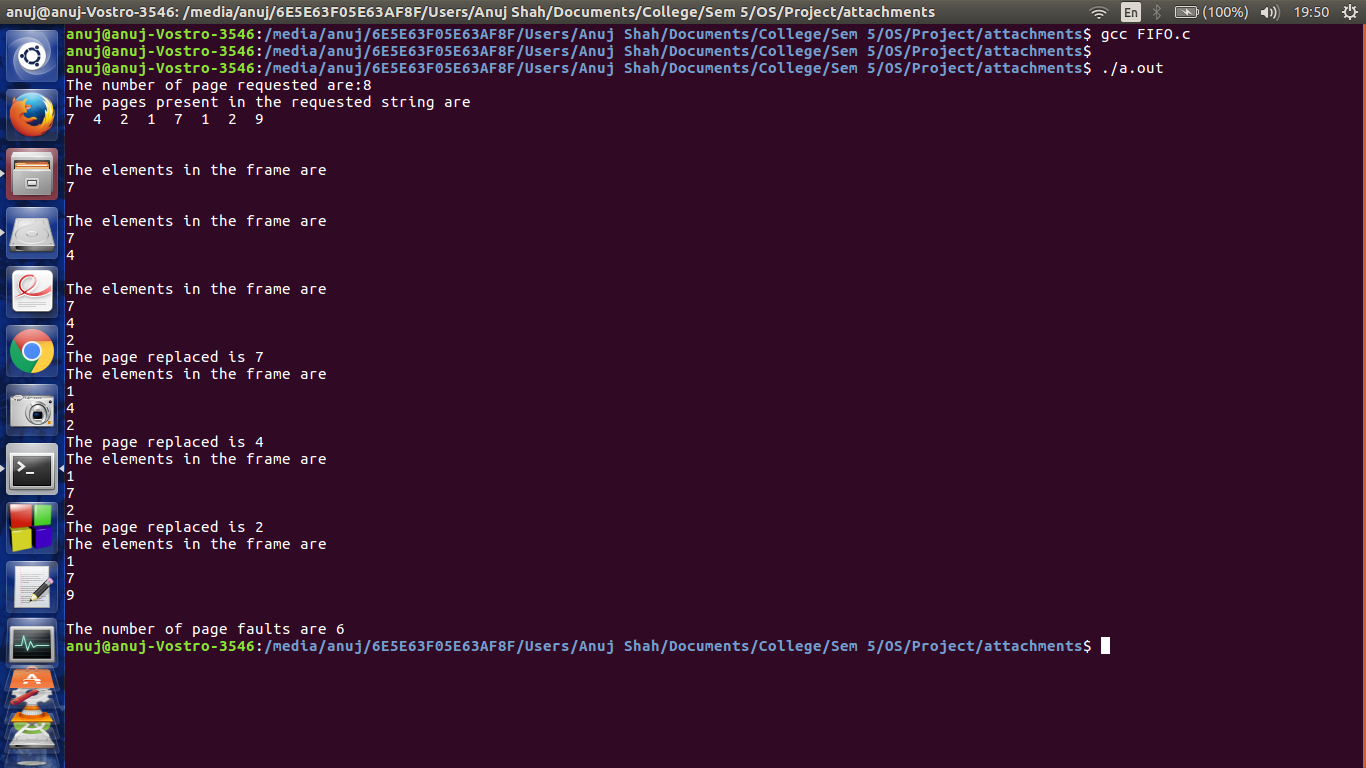
\includegraphics[height=7cm]{FIFO_result.png}
    	\subsection{LFU}
		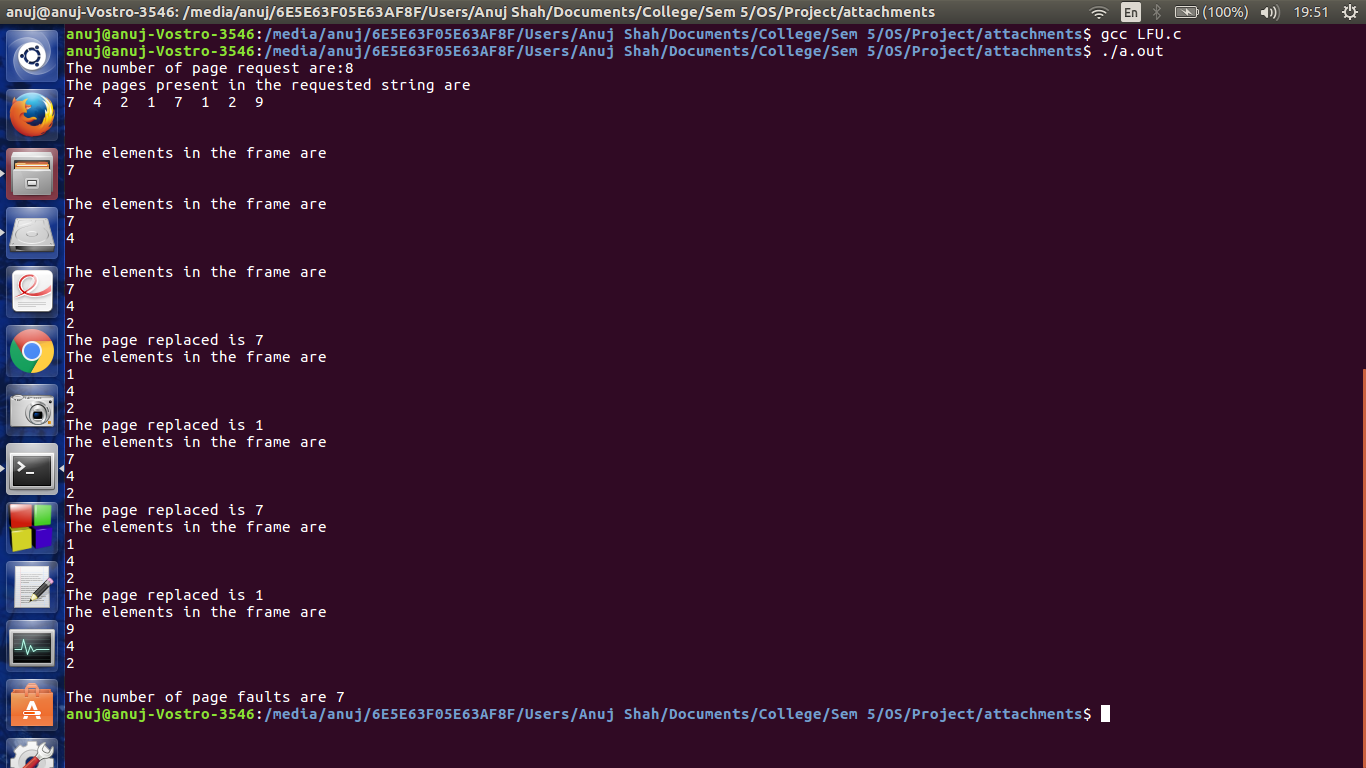
\includegraphics[height=7cm]{LFU_result.png}
		\subsection{LRU Counter}
		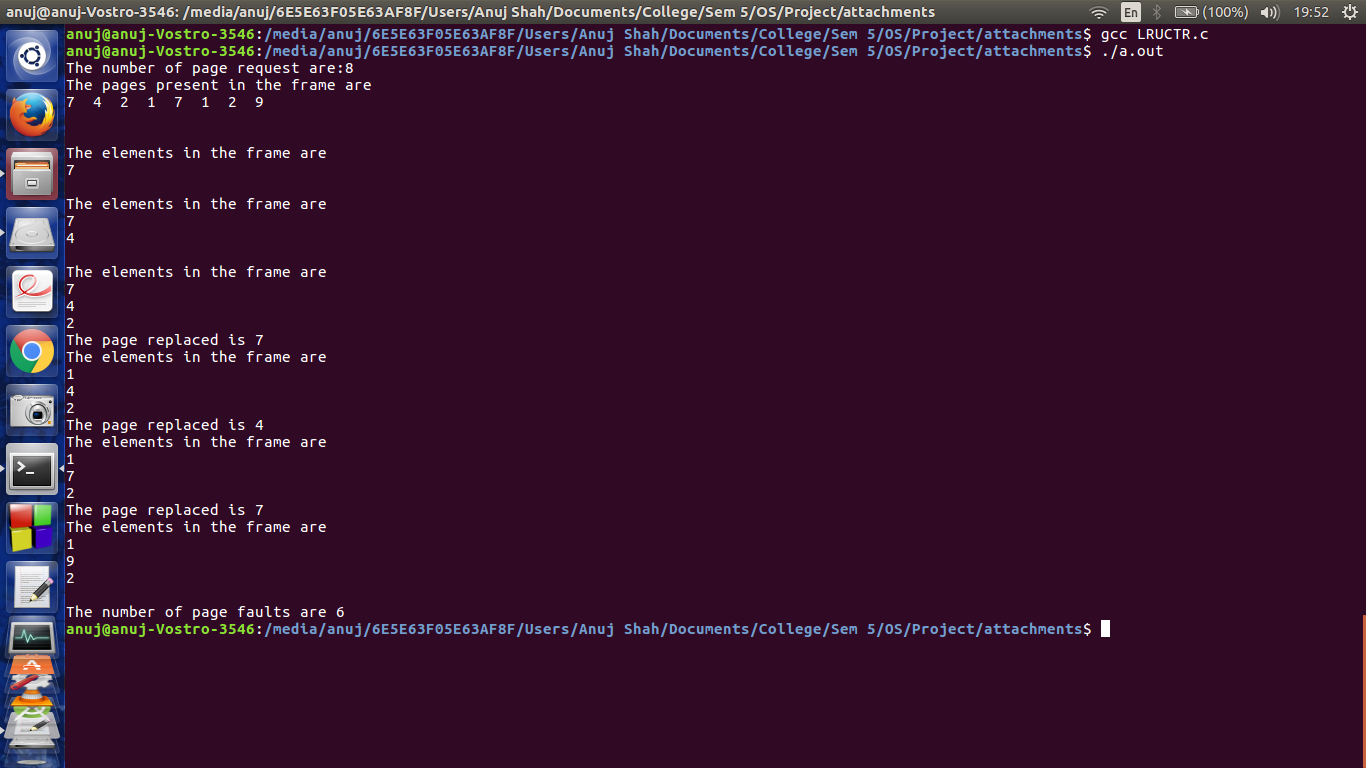
\includegraphics[height=7cm]{LRUCTR_result.png}
		\subsection{LRU Stack}
		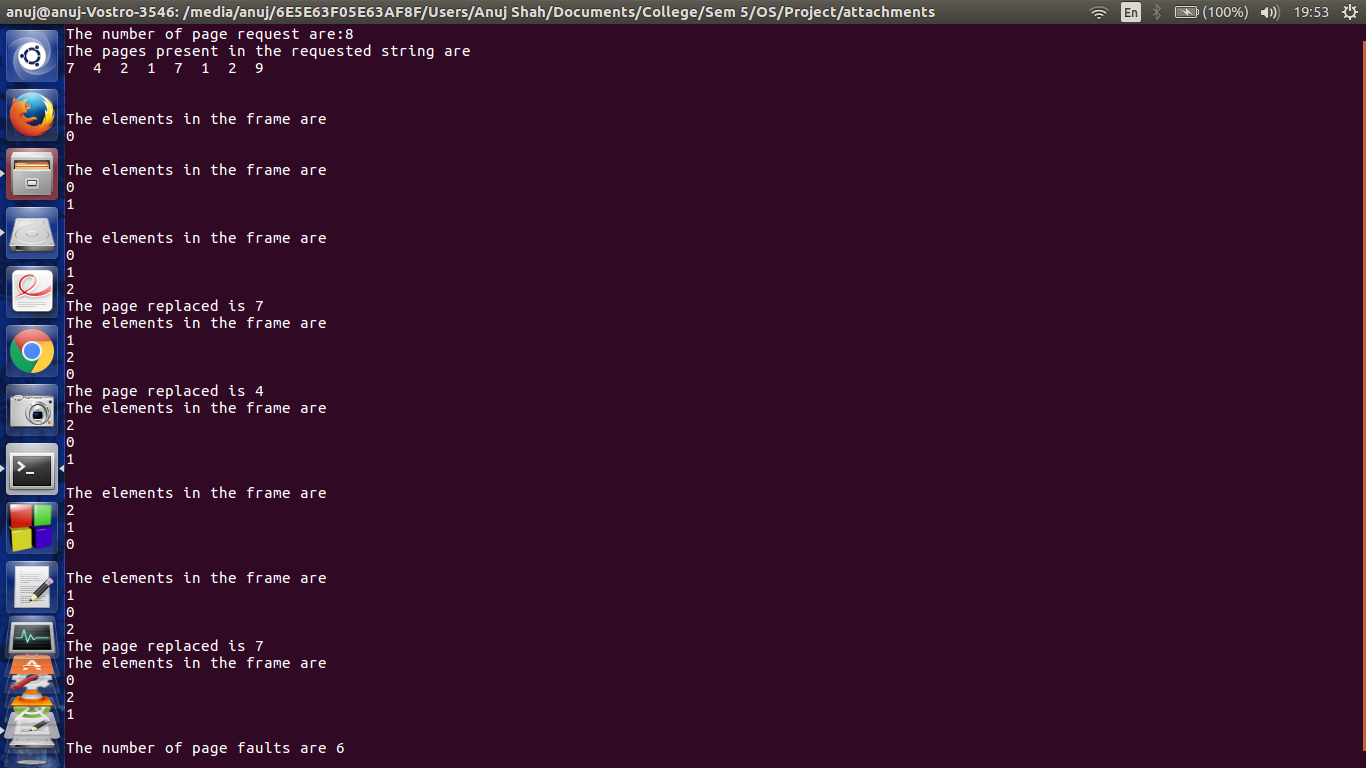
\includegraphics[height=7cm]{LRUstack_result.png}
		\subsection{MFU}
		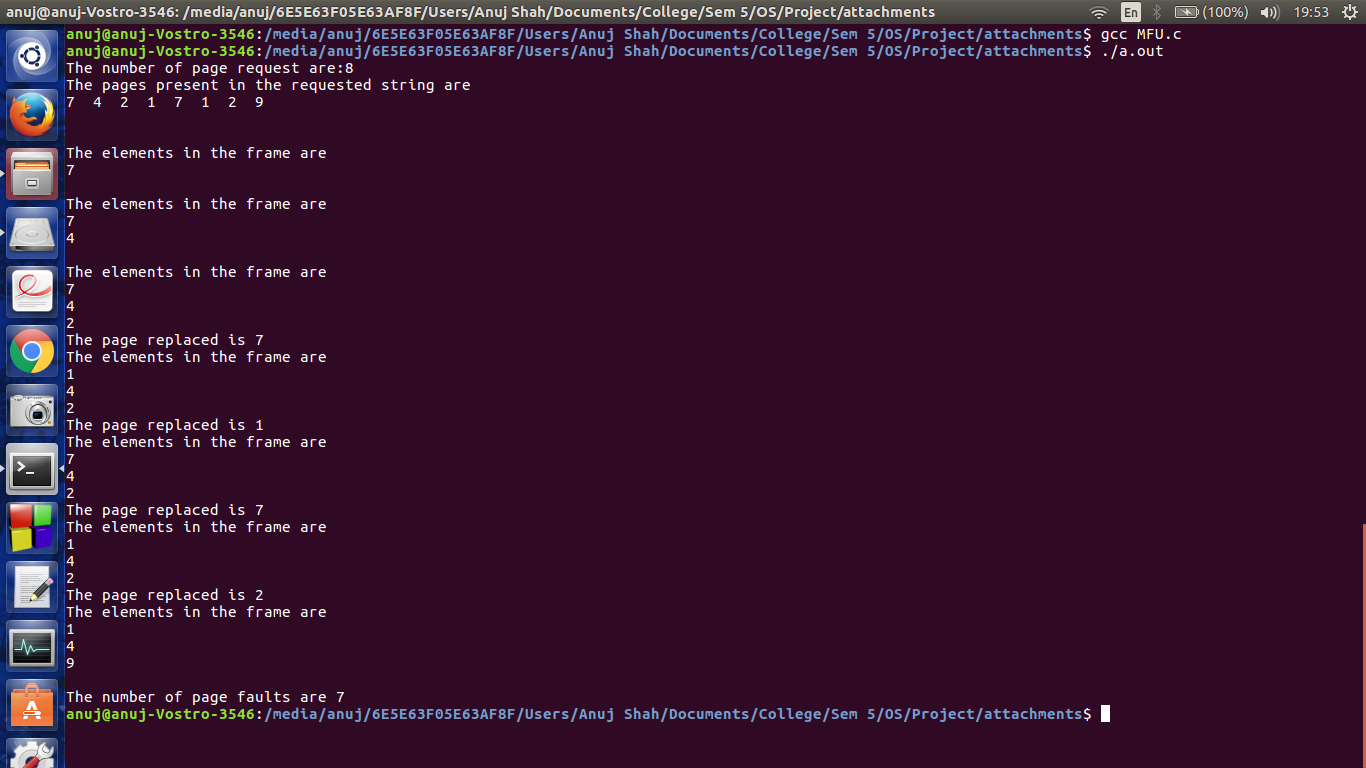
\includegraphics[height=7cm]{MFU_result.png}
	    \subsection{OPT}
		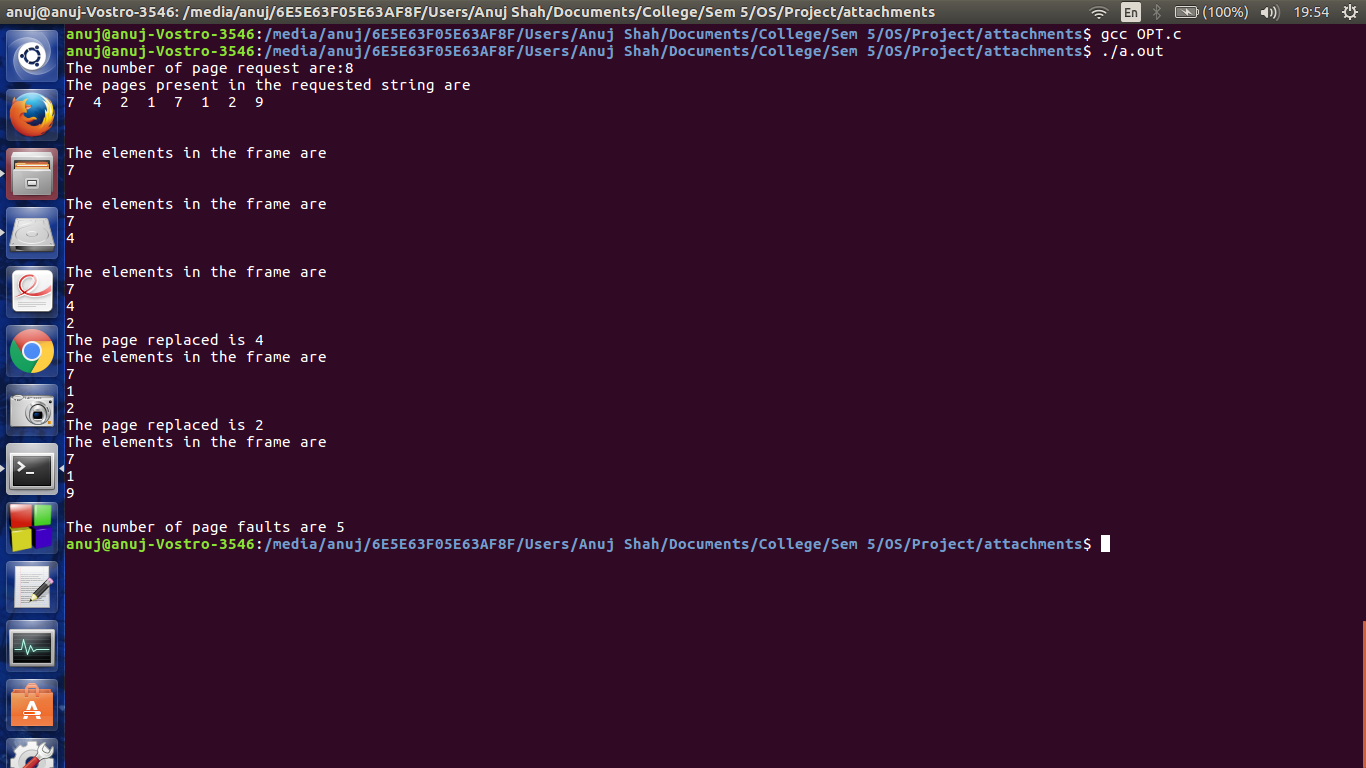
\includegraphics[height=7cm]{OPT_result.png}
		\subsection{Second Chance}
		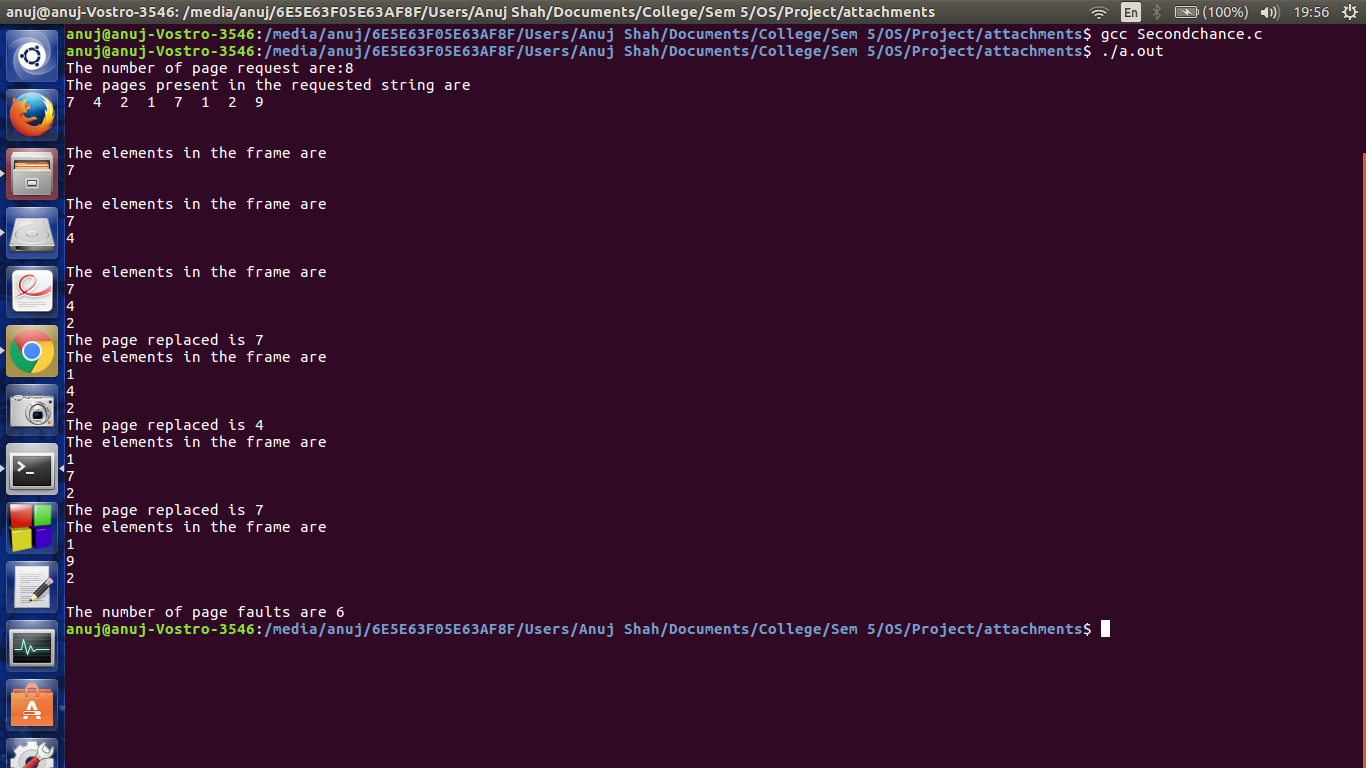
\includegraphics[height=7cm]{Secondchance_result.png}
	\end{flushleft}
	
	\begin{flushleft}
	\section{Technical Specification}
	
	Code Language – C and Python 2.7\\
	Code compatibility – UNIX and Windows\\
	Input – Randomly generated page numbers using Python\\
	Output – Number of page faults and intermediate pages in frame\\
	Data structures used – Stack, Array, Linked list\\
	\pagebreak
	\end{flushleft}	
	\begin{flushleft}
		\section{Analysis of most used Algorithm}
	A table with number of page faults, for each algorithm, with page frame size 2, 3 and 4 is generated as shown in table 1. With 2 page frames, FIFO generates 11 page faults, LRU generates 11 page faults and Optimal generates 8 page faults. Similarly with 3 page frames, FIFO generates 9 page faults, LRU generates 9 page faults and Optimal generates 6 page faults. With 4 page frames, FIFO generates 5 page faults, LRU generates 6 page faults and Optimal generates 5 page faults.
	\end{flushleft}
	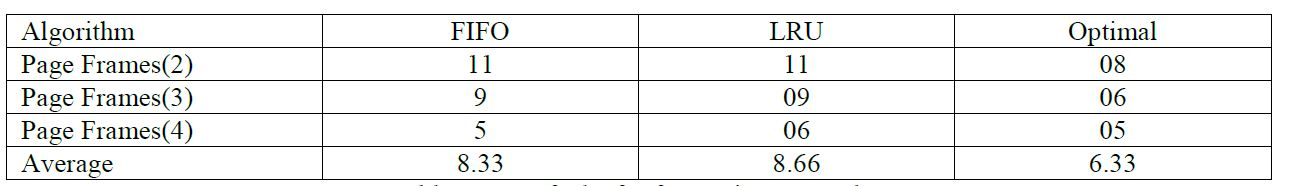
\includegraphics[width=10cm]{Analysis.JPG}\\
	\vspace{2cm}
	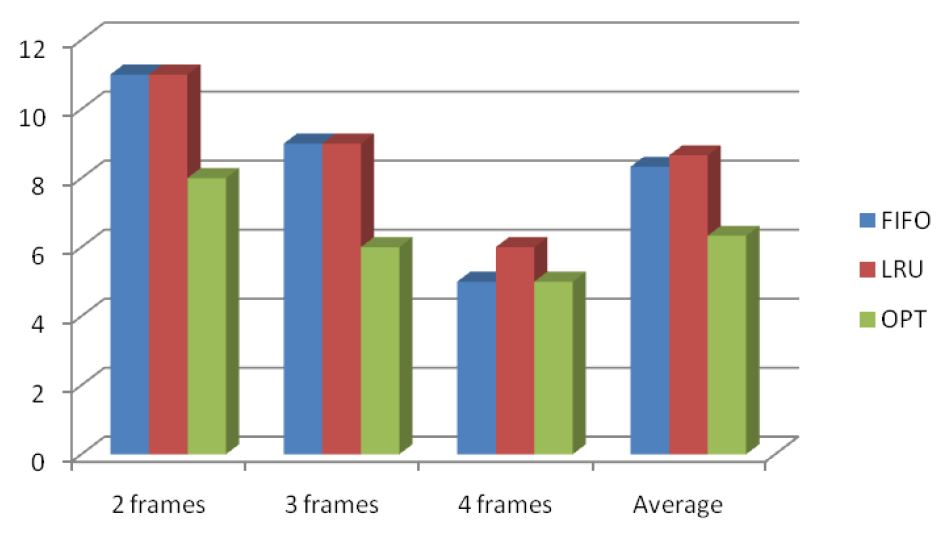
\includegraphics[width=10cm]{Analysis_Graph.JPG}
	\pagebreak
	\begin{flushleft}
		\section{Anamoly of FIFO page replacement algorithm - Bélády's anomaly}
	In computer storage, Bélády's anomaly is the phenomenon in which increasing the number of page frames results in an increase in the number of page faults for certain memory access patterns. This phenomenon is commonly experienced when using the First in First Out (FIFO) page replacement algorithm. 
	
	\end{flushleft}
	\vspace{2cm}
	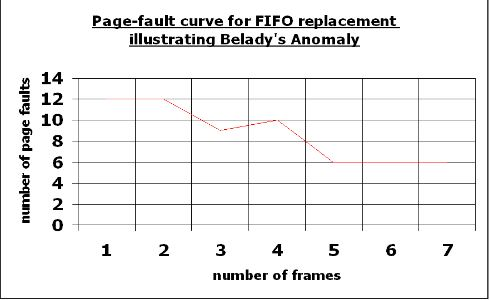
\includegraphics[width=10cm]{FIFO_Analysis.JPG}
	\begin{center}
		Illustration of  Bélády's anomaly
	\end{center}
	
	\pagebreak
	\begin{flushleft}
		\section{References}
		\begin{thebibliography}{10}
			
		\bibitem{1} Operating System internals and Design Principles, 7th ed. Pearson
		\bibitem{2}"LRU Implementations", \url{Cs.jhu.edu}, 2016. [Online]. Available: \url{http://www.cs.jhu.edu/~yairamir/cs418/os6/tsld021.htm}. $[Accessed: 07- Dec- 2016].$\\
		\bibitem{3} "Operating System - Virtual Memory", \url{www.tutorialspoint.com}, 2016. $[Online].$ Available: \url{https://www.tutorialspoint.com/operating_system/os_virtual_memory.htm}. $[Accessed: 07- Dec- 2016].$\\
		\bibitem{4} "Operating Systems", \url{Www2.cs.uregina.ca}, 2016. $[Online]$. Available: \url{http://www2.cs.uregina.ca/~hamilton/courses/330/notes/memory/page_replacement.html}. $[Accessed: 07- Dec- 2016].$\\
		\bibitem{5} "Page replacement algorithm", En.wikipedia.org, 2016. $[Online].$ Available: \url{https://en.wikipedia.org/wiki/Page_replacement_algorithm}. $[Accessed: 07- Dec- 2016]$.\\
		\bibitem{6} "What’s the difference between clock and Second chance page-replacement algorithm?," 2016. [Online]. Available: \url{http://cs.stackexchange.com/questions/29092/whats-the-difference-between-clock-and-second-\\
			chance-page-replacement-algorithm}. Accessed: Dec. 7, 2016.\\
		\bibitem{7}"Page Replacement Algorithm", \url{http://www.cs.utexas.edu/users/witchel/372/lectures/16.PageReplacementAlgos.pdf}, 2016.
		\bibitem{9} Optimal (OPT) Page replacement Algorithm,\url{http://faculty.salina.k-state.edu/tim/ossg/_images/optimal.png} 2016.
		\bibitem{8}Most Frequently Used(MFU) Page replacement Algorithm, \url{http://images.slideplayer.com/20/6026617/slides/slide_56.jpg} 2016.
			
		\end{thebibliography}
	\end{flushleft}
	
		
\end{document}